\begin{exercício}{}{exercício2}
    O princípio ativo do colorante Cl 42555 (violeta crista) é o cátion orgânico monovalente \ce{C[C6H4N(CH3)2]3^+}. O esqueleto desse íon é constituído por três ramos idênticos, como na figura abaixo, o déficit eletrônico responsável pela carga \(+\) podendo ter sido retirado de qualquer um dos três ramos.
    \begin{center}
        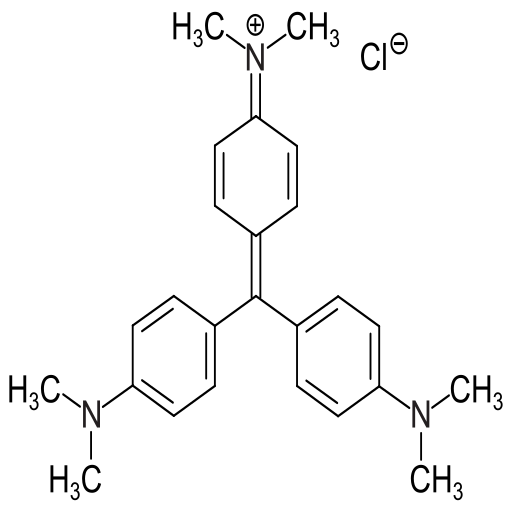
\includegraphics[height=0.15\textheight]{Cl42555.png}
    \end{center}
    Podemos tratar o estado eletrônico desse íon como um sistema de três estados. O hamiltoniano \(H\) não é diagonal na base ortonormal \(\set{\ket{1},\ket{2}, \ket{3}}\) correspondente aos estados das \enquote{configurações clássicas}, pois é possível passar de uma \enquote{configuração clássica} para outra por um efeito quântico denominado efeito túnel que estudaremos futuramente.
    \begin{enumerate}[label=(\alph*)]
        \item Trabalharemos na base de \enquote{configurações clássicas}. Escolheremos a origem das energias tal que tenhamos \(\bra{n}H\ket{n} = 0.\) Temos também \(\bra{1}H\ket{2} = \bra{2}H\ket{3} = \bra{3}H\ket{1} = -A,\) onde \(A > 0\). Escreva a matriz que representa \(H\) nessa base.
        \item Considere os estados \(\ket{\phi_1} = \frac{1}{\sqrt{3}} (\ket{1} + \ket{2} + \ket{3})\) e \(\ket{\phi_2} = \frac1{\sqrt{2}} (\ket{2} - \ket{3}\). Calcule o valor médio da energia e seu desvio padrão para cada um desses estados.
        \item Determine os níveis de energia do sistema. Encontre uma base ortonormal simples. Essa base é única?
    \item Temos \(A \sim \SI{0.75}{eV}.\) Por que o íon tem cor violeta? Lembramos que as cores do espectro da luz branca são, em ordem de energia crescente:
        \begin{enumerate}[label=(\roman*)]
            \item vermelho \(\SI{1.65}{eV} \sim \SI{2.0}{eV}\);
            \item laranja \(\SI{2.0}{eV} \sim \SI{2.1}{eV}\);
            \item amarelo \(\SI{2.1}{eV} \sim \SI{2.3}{eV}\);
            \item verde \(\SI{2.3}{eV} \sim \SI{2.55}{eV}\);
            \item azul \(\SI{2.55}{eV} \sim \SI{2.65}{eV}\); e
            \item violeta \(\SI{2.65}{eV} \sim \SI{3.1}{eV}\).
        \end{enumerate}
        As pares principais de \enquote{cores complementares} que associadas restituem a luz branca são amarelo-violeta, vermelho-verde e azul-laranja.
    \item Substituímos o grupo \ce{N(CH3)2} do ramo superior por um átomo de hidrogênio. Supomos que o único efeito dessa substituição seja de elevar \(\bra{1}H\ket{1}\) de uma certa quantidade \(\Delta > 0\), deixando os outros elementos de \(H\) inalterados. Mostre que \(A\) continua autovalor do hamiltoniano. Quais os outros níveis de energia do novo sistema? O que acontece nos limites \(\Delta \ll A\) e \(\Delta \gg A\)?
    \item Esse íon modificado (colorante Cl 42000, verde de malaquita) absorve em dois comprimentos de onda: \SI{620}{nm} e \SI{450}{nm}. Calcule \(\Delta\) e comente sobre concordância entre teoria e experiência.
    \end{enumerate}
\end{exercício}
\begin{proof}[Resolução]
\end{proof}
